\documentclass[twoside]{amsart}
\usepackage{amssymb,latexsym}
\usepackage{amsfonts}
\usepackage{xspace}
\usepackage{enumerate}
\usepackage{graphics}
\usepackage{fitch}
\newcommand{\Rationals}{\mathbb{Q}{}}
\newcommand{\Reals}{\ensuremath{\mathbb{R}}\xspace}
\newcommand{\Integers}{\ensuremath{\mathbb{Z}{}}\xspace}
\newcommand{\solution}{\textsc{Solution}\xspace}
\newcommand{\problem}{\textsc{Problem}\xspace}
\newcommand{\Blank}{\mathrel{\phantom{=}}}
\newcommand{\ltrue}{\top}
\newcommand{\lfalse}{\bot}
\newcommand{\fOfg}{\ensuremath{f \circ g}\xspace}
\newcommand{\gOff}{\ensuremath{g \circ f}\xspace}
\newcommand{\eps}{\ensuremath{\epsilon}\xspace}
\begin{document}
\title{Answers to Chapter 7 Exercises - A Book of Abstract Algebra}
\author{Michael Welch}
\date{\today}
\maketitle

This document contains selected answers to exercises from chapter 7
of A Book of Abstract Algebra.


\begin{enumerate}[A.]
   \item \textsc{Computing Elements of} $S_6$
   \begin{enumerate}[1]
      \item Consider the following permutations $f$, $g$, and $h$ in $S_6$:
      \begin{align*}
         f & = \begin{pmatrix}
	           1 & 2 & 3 & 4 & 5 & 6 \\
		   6 & 1 & 3 & 5 & 4 & 2
	       \end{pmatrix} \\
	 g & = \begin{pmatrix}
	           1 & 2 & 3 & 4 & 5 & 6 \\
		   2 & 3 & 1 & 6 & 5 & 4
	       \end{pmatrix} \\
	 h & = \begin{pmatrix}
	          1 & 2 & 3 & 4 & 5 & 6 \\
		  3 & 1 & 6 & 4 & 5 & 2
	       \end{pmatrix}
      \end{align*}

      Compute the following: $f^{-1}$, $g^{-1}$, $h^{-1}$, $f \circ g$,
      $g \circ f$.

      \solution 
      \begin{align*}
         f^{-1} & = \begin{pmatrix}
	                1 & 2 & 3 & 4 & 5 & 6 \\
			2 & 6 & 3 & 5 & 4 & 1
	            \end{pmatrix} \\
         g^{-1} & = \begin{pmatrix}
	                1 & 2 & 3 & 4 & 5 & 6 \\
			3 & 1 & 2 & 6 & 5 & 4
	            \end{pmatrix} \\
         h^{-1} & = \begin{pmatrix}
	                1 & 2 & 3 & 4 & 5 & 6 \\
			2 & 6 & 1 & 4 & 5 & 3
	            \end{pmatrix} \\
         f \circ g & = \begin{pmatrix}
	                  1 & 2 & 3 & 4 & 5 & 6 \\
			  1 & 3 & 6 & 2 & 4 & 5
	               \end{pmatrix} \\
         g \circ f & = \begin{pmatrix}
	                  1 & 2 & 3 & 4 & 5 & 6 \\
			  4 & 2 & 1 & 5 & 6 & 3
	               \end{pmatrix}
      \end{align*}

      \item $f \circ (g \circ h)$

      \solution
      \begin{align*}
         f \circ (g \circ h) & = \begin{pmatrix}
	                            1 & 2 & 3 & 4 & 5 & 6 \\
				    6 & 1 & 5 & 2 & 4 & 3
	                         \end{pmatrix}
      \end{align*}

      \item $g \circ h^{-1}$

      \solution
      \begin{align*}
         g \circ h^{-1} & = \begin{pmatrix}
	                       1 & 2 & 3 & 4 & 5 & 6 \\
			       3 & 4 & 2 & 6 & 5 & 1
			    \end{pmatrix}
      \end{align*}

      \item $h \circ g^{-1} \circ f^{-1}$

      \solution
      \begin{align*}
         h \circ g^{-1} \circ f^{-1} & = \begin{pmatrix}
	                                    1 & 2 & 3 & 4 & 5 & 6 \\
					    3 & 4 & 1 & 5 & 2 & 6
	                                 \end{pmatrix}
      \end{align*}

      \item $g \circ g \circ g$

      \solution
      \begin{align*}
         g \circ g \circ g & = \begin{pmatrix}
	                          1 & 2 & 3 & 4 & 5 & 6 \\
				  1 & 2 & 3 & 4 & 5 & 6
	                       \end{pmatrix}
      \end{align*}
   \end{enumerate}

   \item \textsc{Examples of Groups of Permutations}

   \begin{enumerate}[1]
      \item Let $G$ be the subset of $S_4$ consisting of the permutations
      \begin{align*}
         \epsilon & =  \begin{pmatrix}
	                 1 & 2 & 3 & 4 \\
			 1 & 2 & 3 & 4
	              \end{pmatrix}
		      &
         f        & = \begin{pmatrix}
	                 1 & 2 & 3 & 4 \\
			 2 & 1 & 4 & 3
		      \end{pmatrix} \\
         g        & = \begin{pmatrix}
	                 1 & 2 & 3 & 4 \\
			 3 & 4 & 1 & 2
		      \end{pmatrix}
		      &
         h        & = \begin{pmatrix}
	                 1 & 2 & 3 & 4 \\
			 4 & 3 & 2 & 1
		      \end{pmatrix}
      \end{align*}

      Show that $G$ is a group of permutations, and write its table:

      \solution The neutral element is $\epsilon$. Each element is its
      own inverse:

      \begin{center}
      \begin{tabular}{c|cccc}
         $\circ$ & $\epsilon$ &     $f$    &     $g$    &     $h$    \\ \hline
      $\epsilon$ & $\epsilon$ &     $f$    &     $g$    &     $h$    \\
          $f$    &     $f$    & $\epsilon$ &     $h$    &     $g$    \\
	  $g$    &     $g$    &     $h$    & $\epsilon$ &     $f$    \\
	  $h$    &     $h$    &     $g$    &     $f$    & $\epsilon$ 
      \end{tabular}
      \end{center}

      \item List the elements of the cyclic subgroup of $S_6$ generated by
      \begin{align*}
         f &= \begin{pmatrix}
	         1 & 2 & 3 & 4 & 5 & 6 \\
		 2 & 3 & 4 & 1 & 6 & 5
	      \end{pmatrix}
      \end{align*}

      \solution 
      \begin{align*}
         f \circ f & = \begin{pmatrix}
	                  1 & 2 & 3 & 4 & 5 & 6 \\
			  3 & 4 & 1 & 2 & 5 & 6
	               \end{pmatrix} \\
         f \circ f \circ f & = \begin{pmatrix}
	                          1 & 2 & 3 & 4 & 5 & 6 \\
				  4 & 1 & 2 & 3 & 6 & 5
	                       \end{pmatrix} \\
	 f \circ f \circ f \circ f & =
	               \begin{pmatrix}
		          1 & 2 & 3 & 4 & 5 & 6 \\
			  1 & 2 & 3 & 4 & 5 & 6
		       \end{pmatrix}\\
        f \circ f \circ f \circ f \circ f & =
	               \begin{pmatrix}
		          1 & 2 & 3 & 4 & 5 & 6 \\
			  2 & 3 & 4 & 1 & 6 & 5
		       \end{pmatrix} \\
		       & = f
      \end{align*}

      \item Find a four element abelian group subgroup of $S_5$. Write
      its table. 
      
      \solution $S_5$ is the symmetric group on the set  $\{1,2,3,4,5\}$.  Four
      functions $a$, $b$, $c$, $d$ are needed such that $a \circ b = b \circ
      a$, $a \circ c=c \circ a$, $a \circ d=d \circ a$, $b \circ c=c \circ b$,
      $b \circ d=d \circ b$ and $c \circ d=d \circ c$. Let's set up
      all the equations:

      \begin{align*}
         a(b(x)) & = b(a(x)) \\
	 a(c(x)) & = c(a(x)) \\
	 a(d(x)) & = d(a(x)) \\
	 b(c(x)) & = c(b(x)) \\
	 b(d(x)) & = d(b(x)) \\
	 c(d(x)) & = d(c(x)) 
      \end{align*}

      We know that we need a neutral element $\epsilon$. Let's choose
      $a$ to be the neutral element.
      \begin{align*}
         a & = \begin{pmatrix}
	          1 & 2 & 3 & 4 & 5 \\
		  1 & 2 & 3 & 4 & 5
	       \end{pmatrix}
      \end{align*}

      Let's choose $b$ as such:
      \begin{align*}
         b & = \begin{pmatrix}
	          1 & 2 & 3 & 4 & 5 \\
		  2 & 3 & 4 & 1 & 5
	       \end{pmatrix}
      \end{align*}

      Then let's choose $c= b \circ b$:
      \begin{align*}
         c & = \begin{pmatrix}
	          1 & 2 & 3 & 4 & 5 \\
		  3 & 4 & 1 & 2 & 5
	       \end{pmatrix}
      \end{align*}

      And finally $d = c \circ b$
      \begin{align*}
         d & = \begin{pmatrix}
	          1 & 2 & 3 & 4 & 5 \\
		  4 & 1 & 2 & 3 & 5
	       \end{pmatrix}
      \end{align*}

      The table is then
      \begin{center}
      \begin{tabular}{c|cccc}
         $\circ$ & $a$ & $b$ & $c$ & $d$ \\ \hline
	     $a$ & $a$ & $b$ & $c$ & $d$ \\
	     $b$ & $b$ & $c$ & $d$ & $a$ \\
	     $c$ & $c$ & $d$ & $a$ & $b$ \\
	     $d$ & $d$ & $a$ & $b$ & $c$
      \end{tabular}
      \end{center}

      This group is a cyclic group generated by $b$.

      \item The subgroup of $S_5$ generated by 
      \begin{align*}
         f & = \begin{pmatrix}
	          1 & 2 & 3 & 4 & 5 \\
		  2 & 1 & 3 & 4 & 5 \\
	       \end{pmatrix}
	       &
	 g & = \begin{pmatrix}
	          1 & 2 & 3 & 4 & 5 \\
		  1 & 2 & 4 & 5 & 3 \\
	       \end{pmatrix}
      \end{align*}

      has six elements. List them, then write the table of this group.
      \begin{align*}
         \epsilon & = \begin{pmatrix}
	                 1 & 2 & 3 & 4 & 5 \\
			 1 & 2 & 3 & 4 & 5
		      \end{pmatrix}
		      &
         f & = \begin{pmatrix}
	          1 & 2 & 3 & 4 & 5 \\
		  2 & 1 & 3 & 4 & 5 \\
	       \end{pmatrix} \\
	 g & = \begin{pmatrix}
	          1 & 2 & 3 & 4 & 5 \\
		  1 & 2 & 4 & 5 & 3 \\
	       \end{pmatrix}
	       &
	 h & = \begin{pmatrix}
	          1 & 2 & 3 & 4 & 5 \\
		  2 & 1 & 4 & 5 & 3 \\
	       \end{pmatrix} \\
	 k & = \begin{pmatrix}
	          1 & 2 & 3 & 4 & 5 \\
		  1 & 2 & 5 & 3 & 4 \\
	       \end{pmatrix}
	       &
	 l & = \begin{pmatrix}
	          1 & 2 & 3 & 4 & 5 \\
		  2 & 1 & 5 & 3 & 4 \\
	       \end{pmatrix}
      \end{align*}

      Here is the table:
      \begin{center}
      \begin{tabular}{c|cccccc}
      $\circ$ & $\epsilon$ & $f$ & $g$ & $h$ & $k$ & $l$ \\ \hline
    $\epsilon$& $\epsilon$ & $f$ & $g$ & $h$ & $k$ & $l$ \\
          $f$ & $f$ & $\epsilon$ & $h$ & $g$ & $l$ & $k$ \\
	  $g$ & $g$ & $h$ & $k$ & $l$ & $\epsilon$ & $f$ \\
	  $h$ & $h$ & $g$ & $l$ & $k$ & $f$ & $\epsilon$ \\
	  $k$ & $k$ & $l$ & $\epsilon$ & $f$ & $g$ & $h$ \\
	  $l$ & $l$ & $k$ & $f$ & $\epsilon$ & $h$ & $g$
      \end{tabular}
      \end{center}

   \end{enumerate}

   \vspace{5pt}
   \item \textsc{Groups of Permutations of} \Reals

   In each of the following, $A$ is a subset of \Reals and $G$ is a set of 
   permutations of $A$. Show that $G$ is a subgroup of $S_A$, and write
   the table of $G$.

   \begin{enumerate}[1]
      \item $A$ is the set of all $x \in \Reals$ such that $x \ne 0,1$.
      $G = \{\epsilon, f, g\}$, where $f(x) = 1/(1-x)$ and 
      $g(x)=(x-1)/x$.

      \solution To prove that $G$ is a subgroup we must show that it
      is closed with respect to $\circ$ and it is closed with 
      respect to function inverses.

      By definition $f \circ \epsilon = \epsilon \circ f = f \in G$.
      Likewise, $g \circ \epsilon = \epsilon \circ g = g \in G$.
      \begin{align*}
         f(g(x)) & = f\left(\frac{x-1}{x}\right) & 
	 g(f(x)) & = g\left(\frac{1}{1-x}\right) \\
                 & = \frac{1}{1-\displaystyle \frac{x-1}{x}} &
		 & = \frac{\displaystyle\frac{1}{1-x}-1}
		          {\displaystyle\frac{1}{1-x}} \\
	         & = \frac{x}{x-(x-1)} &
		 & = \frac{1-(1-x)}{1} \\
		 & = \frac{x}{x-x+1} &
		 & = \frac{1-1+x}{1} \\
		 & = x &
		 & = x
      \end{align*}
      This tells us that
      it is closed with respect to function inverses since
      $f^{-1}=g$ and $g^{-1}=f$.
      
      Now what about $f \circ f$ and $g \circ g$
      \begin{align*}
         f(f(x)) & = f\left(\frac{1}{1-x}\right) \\
	         & = \frac{1}{1-\displaystyle\frac{1}{1-x}}\\
		 & = \frac{1-x}{1-x-1} \\
		 & = \frac{1-x}{-x} \\
		 & = \frac{x-1}{x} \\
		 & = g(x) \\
	 g(g(x)) & = g\left(\frac{x-1}{x}\right) \\
	         & = \frac{\displaystyle\frac{x-1}{x}-1}
		          {\displaystyle\frac{x-1}{x}} \\
	         & = \frac{x-1-x}{x-1} \\
		 & = \frac{-1}{x-1} \\
		 & = \frac{1}{1-x} \\
		 & = f(x)
      \end{align*}
      

      Therefore $f \circ g = g \circ f = \epsilon$, $f \circ f = g$,
      and $g \circ g = f$. Thus $G$ is
      closed with respect to $\circ$. The table of $G$ is
      \begin{center}
      \begin{tabular}{c|ccc}
         $\circ$ & $\epsilon$ & $f$ & $g$ \\ \hline
      $\epsilon$ & $\epsilon$ & $f$ & $g$ \\
             $f$ & $f$ & $g$ & $\epsilon$ \\
	     $g$ & $g$ & $\epsilon$ & $f$
      \end{tabular}
      \end{center}

      \item $A$ is the set of all the nonzero real numbers. $G = \{
      \epsilon, f, g, h\}$, where $f(x)=1/x$, $g(x)=-x$, and $h(x)=-1/x$.

      \solution $G$ is closed with respect to inverses:

      $f^{-1}=f$: 
      \begin{proof}
	 \begin{align*}
	    [f \circ f](x) &= f(f(x)) \\
	                   &= f(1/x) \\
			   &= 1/(1/x) \\
			   &= x \\
			   &= \epsilon(x) \qedhere
	 \end{align*}
      \end{proof}

      $g^{-1}=g$: 
      \begin{proof}
	 \begin{align*}
	    [g \circ g](x) &= g(g(x)) \\
	                   &= g(-x) \\
			   &= -(-x) \\
			   &= x \\
			   &= \epsilon(x) \qedhere
	 \end{align*}
      \end{proof}

      $h^{-1}=h$: 
      \begin{proof}
	 \begin{align*}
	    [h \circ h](x) &= h(-1/x) \\
	                   &= -1/(-1/x) \\
			   &= x \\
			   &= \epsilon(x) \qedhere
	 \end{align*}
      \end{proof}

      Therefore $G$ is closed with respect to inverses. Next we will show $G$
      is closed with respect to $\circ$. Need to compute $f \circ f$, $f \circ
      g$, $f \circ h$, $g \circ f$, $g \circ g$, $g \circ h$, $h \circ f$, $h
      \circ g$, $h \circ h$.

      $f \circ f = \epsilon$, $f \circ g = h$, $f \circ h = g$, 
      $g \circ f = h$, $g \circ g = \epsilon$, $g \circ h = f$,
      $h \circ f = g$, $h \circ g = f$, $h \circ h = \epsilon$. The
      table of $G$ is
      \begin{center}
      \begin{tabular}{c|cccc}
        $\circ$ & $\epsilon$ & $f$ & $g$ & $h$ \\ \hline
      $\epsilon$& $\epsilon$ & $f$ & $g$ & $h$ \\
            $f$ & $f$ & $\epsilon$ & $h$ & $g$ \\
	    $g$ & $g$ & $h$ & $\epsilon$ & $f$ \\
	    $h$ & $h$ & $g$ & $f$ & $\epsilon$
      \end{tabular}
      \end{center}

      \item $A$ is the set of all the real numbers $x \ne 0,1$. $G =
      \{\epsilon, f, g, h, j, k \}$, where $f(x)=1-x$, $g(x)=1/x$,
      $h(x)=1/(1-x)$, $j(x)=(x-1)/x$, and $k(x)=x/(x-1)$.

      \solution It is trivial to show that $f^{-1}=f$, $g^{-1}=g$,
      $h^{-1}=j$, $j^{-1}=h$, and $k^{-1}=k$:
      \begin{align*}
         [f \circ f](x) &= f(f(x))  & [g \circ g](x) &= g(g(x)) \\
	           &= f(1-x)        &                &= g(1/x) \\
		   &= 1 - (1-x)     &                &= 1/(1/x) \\
		   &= x             &                &= x\\
		   &= \epsilon(x)   &                &= \epsilon(x)  \\
         [h \circ j](x) &= h(j(x))  & [j \circ h](x) &= j(h(x)) \\
	           &= h((x-1)/x)    &                &= j(1/(1-x)) \\
		   &= 1/(1-((x-1)/x)) &             &= ((1/(1-x))-1)/(1/(1-x))\\
		   &= x/(x-(x-1))   &                &= (1-(1-x))/1\\
		   &= x             &                &= x\\
		   &= \epsilon(x)   &                &= \epsilon(x) \\
      \end{align*}
      \begin{align*}
         [k \circ k](x) &= k(k(x)) \\
	           &= k(x/(x-1))   \\
		   &= (x/(x-1))/((x/x-1)-1) \\
		   &= x/(x-(x-1)) \\
		   &= x \\
		   &= \epsilon(x)
      \end{align*}

      Therefore $G$ is closed with respect to inverses. Now we need
      to compute all the other combinations of $\circ$:     
      \begin{itemize}
         \item $f(g(x)) = f(1/x) = 1-(1/x) = (x-1)/x = j(x)$,
         \item $f(h(x)) = f(1/(1-x)) = 1-(1/(1-x)) = x/(x-1) = k(x)$
	 \item $f(j(x)) = f((x-1)/x) = 1-((x-1)/x) = 1/x = g(x)$
	 \item $f(k(x)) = f(x/(x-1)) = 1-(x/(x-1)) = 1/(1-x) = h(x)$
	 \item $g(f(x)) = g(1-x) = 1/(1-x) = h(x)$
         \item $g(h(x)) = g(1/(1-x)) = 1-x = f(x)$
	 \item $g(j(x)) = g((x-1)/x) = x/(x-1) = k(x)$
	 \item $g(k(x)) = g(x/(x-1)) = (x-1)/x = j(x)$
	 \item $h(f(x)) = h(1-x) = 1/(1-(1-x)) = 1/x = g(x)$
	 \item $h(g(x)) = h(1/x) = 1/(1-(1/x)) = x/(x-1) = k(x)$
	 \item $h(h(x)) = h(1/(1-x)) = 1/(1-(1/(1-x))) = (x-1)/x = j(x)$
	 \item $h(k(x)) = h(x/(x-1)) = 1/(1-(x/(x-1))) = 1-x = f(x)$
	 \item $j(f(x)) = j(1-x) = ((1-x)-1)/(1-x) = x/(x-1) = k(x)$
	 \item $j(g(x)) = j(1/x) = ((1/x)-1)/(1/x) = 1-x = f(x)$
	 \item $j(j(x)) = j((x-1)/x) = (((x-1)/x)-1)/((x-1)/x) = 1/(1-x)=h(x)$
	 \item $j(k(x)) = j(x/(x-1)) = ((x/(x-1))-1)/(x/(x-1)) = 1/x = g(x)$
	 \item $k(f(x)) = k(1-x) = (1-x)/(1-x-1) = (x-1)/x= j(x)$
	 \item $k(g(x)) = k(1/x) = (1/x)/((1/x)-1) = 1/(1-x) = h(x)$
	 \item $k(h(x)) = k(1/(1-x)) = (1/(1-x))/((1/(1-x))-1) = 1/x = g(x)$
	 \item $k(j(x)) = k((x-1)/x) = ((x-1)/x)/(((x-1)/x)-1) = 1-x = f(x)$
      \end{itemize}

      Therefore $G$ is closed with respect to $\circ$ and here is the
      table of $G$:

      \begin{center}
      \begin{tabular}{c|cccccc}
         $\circ$ & $\epsilon$ & $f$ & $g$ & $h$ & $j$ & $k$ \\ \hline
	$\epsilon$& $\epsilon$& $f$ & $g$ & $h$ & $j$ & $k$ \\
	     $f$ & $f$ & $\epsilon$ & $j$ & $k$ & $g$ & $h$ \\
	     $g$ & $g$ & $h$ & $\epsilon$ & $f$ & $k$ & $j$ \\
	     $h$ & $h$ & $g$ & $k$ & $j$ & $\epsilon$ & $f$ \\
	     $j$ & $j$ & $k$ & $f$ & $\epsilon$ & $h$ & $g$ \\
	     $k$ & $k$ & $j$ & $h$ & $g$ & $f$ & $\epsilon$
      \end{tabular}
      \end{center}

      \item $A$ is the set of all the real numbers $x \ne 0,1,2$.
      $G$ is the subgroup of $S_A$ generated by $f(x)=2-x$ and 
      $g(x)=2/x$. ($G$ has eight elements. List them, and write
      the table of $G$.)

      \solution The eight elements are
      \begin{enumerate}[(1)]
         \item $f(x)=2-x$
	 \item $g(x)=2/x$ 
	 \item $\epsilon(x)=f(f(x))=f(2-x)=2-(2-x)=x$
	 \item $h(x)=f(g(x))=f(2/x)=2-(2/x)=2(x-1)/x$
	 \item $j(x)=g(f(g(x))) = 2/(2(x-1)/x) = x/(x-1)$
	 \item $k(x)=f(g(f(g(x)))) = 2 - (x/(x-1)) = (x-2)/(x-1)$
	 \item $l(x)=g(f(g(f(g(x))))) = 2/((x-2)/(x-1)) = 2(x-1)/(x-2)$
	 \item $m(x)=f(g(f(g(f(g(x)))))) = 2 - 2(x-1)/(x-2) = 2/(2-x)$
      \end{enumerate}

      The table of $G$ is
      \begin{center}
      \begin{tabular}{c|cccccccc}
         $\circ$ & \eps & $f$ & $g$ & $h$ & $j$ & $k$ & $l$ & $m$ \\ \hline
	  $\eps$ & \eps & $f$ & $g$ & $h$ & $j$ & $k$ & $l$ & $m$ \\
	     $f$ &  $f$ & \eps& $h$ & $g$ & $k$ & $j$ & $m$ & $l$ \\
	     $g$ &  $g$ & $m$ & \eps& $j$ & $h$ & $l$ & $k$ & $f$ \\
	     $h$ &  $h$ & $l$ & $f$ & $k$ & $g$ & $m$ & $j$ & \eps\\
      \end{tabular}
      \end{center}

      \dots and so on.
   \end{enumerate}

   \item \textsc{A Cyclic Group of Permutations}

   \noindent For each integer $n$, define $f_n$ by $f_n(x)=x+n$.
   \begin{enumerate}[1]
      \item Prove: For each integer $n$, $f_n$ is a permutation of \Reals,
      that is, $f_n \in S_{\mathbb{R}}$.

      \solution We must show that $f_n$ is bijective (that is it is
       injective and surjective) from \Reals to \Reals.

      $f_n$ is injective. 
      \begin{proof}
         Suppose we have some $a,b \in \Reals$ such that
	  $f_n(a)=f_n(b)$. Then $a+n=b+n$ and $a=b$.
      \end{proof}
      $f_n$ is surjective.
      \begin{proof}
         For all $y \in \Reals$, $y=f(x)$ for $x=y-n$.
      \end{proof}

      \item Prove that $f_n \circ f_m = f_{n+m}$ and $f_n^{-1} = f_{-n}$.

      $f_n \circ f_m = f_{n+m}$.
      \begin{proof}
      \begin{align*}
          [f_n \circ f_m](x) &= f_n(f_m(x)) & f_{n+m} &= x + (n+m) \\
	                     &= f_n(x + m) \\
			     &= x + m + n \\
			     &= x + (n+m) \qedhere
      \end{align*}
      \end{proof}
      $f_n^{-1} = f_{-n}$
      \begin{proof}
      \begin{align*}
         [f_n \circ f_{-n}](x) &= f_n(f_{-n}(x)) \\
	                       &= f_n(x + (-n))  \\
			       &= x + (-n) + n \\
			       &= x \\
			       &= \eps(x) \qedhere
      \end{align*}
      \end{proof}

      \item Let $G=\{f_n : n \in \Integers\}$. Prove that $G$ is a subgroup
      of $S_{\Reals}$.

      $G$ is closed with respect to $\circ$.
      \begin{proof}
      By part 2 we know that $f_n \circ f_m = f_{n+m}$ and $n+m \in \Integers$.
      \end{proof}

      $G$ is closed with respect to inverses.
      \begin{proof}
      By part 2 we know that $f_n^{-1} = f_{-n}$ and we know $-n \in \Integers$.
      \end{proof}

      We also know by part 1 that $f_n : \Reals \to \Reals$. Therefore 
      $G$ is a subgroup of $S_{\mathbb{R}}$.

      \vspace{5pt}
      \item Prove that $G$ is cyclic. (Indicate a generator of $G$.)
      
      \solution $G$ is $\langle f_1 \rangle$
      \begin{proof}
      We must show that for any element $m \in \Integers$ we can 
      generate $f_m$ from $f_1$. Let $m$ be greater than 0. Then we can
      generate $f_m$ by
      \[
         f_m = \underbrace{f_1 \circ f_1 \circ f_1 \cdots f_1 \circ f_1}_{
	          m \text{ factors}} 
      \]

      Next let $m$ be less than 0. Then we can generate it by
      \[
         f_m = \underbrace{f_{-1} \circ f_{-1} \cdots f_{-1}}_{
	          |m| \text{ factors}}
      \]

      Finally, let m = 0. Then $f_0 = f_1 \circ f_{-1} = \epsilon$.
      We have now shown how to generate all the elements in 
      $\{f_n : n \in Integers\}$ using $f_1$.
      \end{proof}


   \end{enumerate}

   \item \textsc{A Subgroup of} $S_\mathbb{R}$

   \noindent For any pair of real numbers $a \ne 0$ and $b$, define a function
   $f_{a,b}$ as follows:
   \[
      f_{a,b} = ax + b
   \]

   \begin{enumerate}[1]
      \item Prove that $f_{a,b}$ is a permutation of \Reals, that is,
      $f_{a,b} \in S_\mathbb{R}$.

      \solution First observe that $f_{a,b} : \Reals \to \Reals$. 
      Choose some $x \in \Reals$. Observe that $f_{a,b} = ax + b$
      is defined and is an element of \Reals. 

      Next we will show that $f_{a,b}$ is both injective and surjective
      and therefore is a permutation of $S_\Reals$.

      \begin{proof}
      $f_{a,b}$ is injective:
         Suppose $f_{a,b}(s) = f_{a,b}(t)$. Then $as+b = at+b$, and
	 $as=at$ and $s=t$ (we know $a \ne 0$).

      $f_{a,b}$ is surjective:
         For all $y \in \Reals$, $y=f_{a,b}(x)$ for $x = (y-b)/a$.

      Therefore $f_{a,b}$ is a permutation of $S_\Reals$.
      \end{proof}

      \item Prove that $f_{a,b} \circ f_{c,d} = f_{ac,ad+b}$.

      \begin{proof}
      \begin{align*}
         [f_{a,b} \circ f_{c,d}](x) &= f_{a,b}(cx+d) \\
	                            &= a(cx+d) + b \\
				    &= acx + (ad+b) \\
				    &= f_{ac,ad+b}
      \end{align*}
      \end{proof}

      \item Prove that $f_{a,b}^{-1} = f_{1/a,-b/a}$.

      We can prove this by calculating $f_{a,b} \circ f_{1/a,-b/a}$.
      \begin{proof}
      \begin{align*}
          [f_{a,b} \circ f_{1/a,-b/a}](x) &= f_{a,b}(x/a+(-b/a)) \\
	                                  &= a(x/a+(-b/a))+b \\
					  &= (x-b)+b \\
					  &= x \\
					  &= \eps(x) \qedhere
      \end{align*}
      \end{proof}

      \item Let $G=\{f_{a,b} : a \in \Reals, b \in \Reals, a \ne 0 \}$.
      Show that $G$ is a subgroup of $S_\Reals$.

      \begin{proof}
      $f_{a,b}$ is closed with respect to $\circ$ and with respect to 
      inverses as shown in part 2 and part 3.
      \end{proof}

   \end{enumerate}

   \item \textsc{Symmetries of Geometric Figures}

   \begin{enumerate}[1]
      \item Let $G$ be the group of symmetries of the regular hexagon. List
      the elements of $G$ (there are 12 of them), then write the table of $G$.

      \begin{center}
      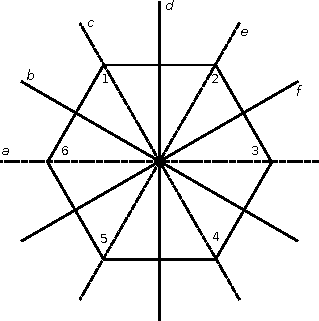
\includegraphics{img/chap7f.pdf}
      \end{center}

      \solution 

      \begin{align*}
	 R_0 & = \begin{pmatrix}
		   1 & 2 & 3 & 4 & 5 & 6 \\
		   1 & 2 & 3 & 4 & 5 & 6
		 \end{pmatrix}
		 &
	 R_1 & = \begin{pmatrix}
		   1 & 2 & 3 & 4 & 5 & 6 \\
		   2 & 3 & 4 & 5 & 6 & 1
		 \end{pmatrix} \\
	 R_2 & = \begin{pmatrix}
		   1 & 2 & 3 & 4 & 5 & 6 \\
		   3 & 4 & 5 & 6 & 1 & 2
		 \end{pmatrix}
		 &
	 R_3 & = \begin{pmatrix}
		   1 & 2 & 3 & 4 & 5 & 6 \\
		   4 & 5 & 6 & 1 & 2 & 3
		 \end{pmatrix} \\
	 R_4 & = \begin{pmatrix}
		   1 & 2 & 3 & 4 & 5 & 6 \\
		   5 & 6 & 1 & 2 & 3 & 4
		 \end{pmatrix}
		 &
	 R_5 & = \begin{pmatrix}
		   1 & 2 & 3 & 4 & 5 & 6 \\
		   6 & 1 & 2 & 3 & 4 & 5
		 \end{pmatrix} \\
	 R_6 & = \begin{pmatrix}
		   1 & 2 & 3 & 4 & 5 & 6 \\
		   5 & 4 & 3 & 2 & 1 & 6
		 \end{pmatrix}
		 &
	 R_7 & = \begin{pmatrix}
		   1 & 2 & 3 & 4 & 5 & 6 \\
		   6 & 5 & 4 & 3 & 2 & 1
		 \end{pmatrix} \\
	 R_8 & = \begin{pmatrix}
		   1 & 2 & 3 & 4 & 5 & 6 \\
		   1 & 6 & 5 & 4 & 3 & 2
		 \end{pmatrix}
		 &
	 R_{10} & = \begin{pmatrix}
		   1 & 2 & 3 & 4 & 5 & 6 \\
		   3 & 2 & 1 & 6 & 5 & 4
		 \end{pmatrix} \\
	 R_{11} & = \begin{pmatrix}
		   1 & 2 & 3 & 4 & 5 & 6 \\
		   4 & 3 & 2 & 1 & 6 & 5
		 \end{pmatrix}
		 &
	 R_9 & = \begin{pmatrix}
		   1 & 2 & 3 & 4 & 5 & 6 \\
		   2 & 1 & 6 & 5 & 4 & 3
		 \end{pmatrix}
      \end{align*}

      \vspace{5pt}
      \item Let $G$ be the group of symmetries of the rectangle. List the
      elements of $G$ (there are four of them), and write the table of $G$.

      \solution Imagine a rectangle with vertices labeled 1,2,3,4 stating
      in the upper left corner and going clockwise.

      \begin{align*}
         R_0 &= \begin{pmatrix}
	           1 & 2 & 3 & 4 \\
		   1 & 2 & 3 & 4
		\end{pmatrix}
		&
         R_1 &= \begin{pmatrix}
	           1 & 2 & 3 & 4 \\
		   3 & 4 & 1 & 2
		\end{pmatrix} \\
         R_2 &= \begin{pmatrix}
	           1 & 2 & 3 & 4 \\
		   4 & 3 & 2 & 1
		\end{pmatrix}
		&
         R_3 &= \begin{pmatrix}
	           1 & 2 & 3 & 4 \\
		   2 & 1 & 4 & 3
		\end{pmatrix} \\
      \end{align*}

      \item List the symmetries of the letter \textbf{Z} and give
      the table of this group of symmetries. Do the same for the letters
      \textbf{V} and \textbf{H}.

      \solution The letter \textbf{Z} has two symmetries the rotations of
      $180^\circ$ and $360^\circ$. We will number the 4 vertices 
      1 thru 4 with 1 in the upper left, 2 the upper right, 3 is lower left and
      4 is lower right. Then the permutations are:
      \begin{align*}
         \text{\textbf{Z}}_0 &= \begin{pmatrix}
	                        1 & 2 & 3 & 4 \\
				1 & 2 & 3 & 4
				\end{pmatrix}
				&
	 \text{\textbf{Z}}_1 &= \begin{pmatrix}
	                        1 & 2 & 3 & 4 \\
				4 & 3 & 2 & 1
				\end{pmatrix}
      \end{align*}
      And the table of \textbf{Z} is
      \begin{tabular}{c|cc}
        $\circ$ & $\textbf{Z}_0$ & $\textbf{Z}_1$ \\ \hline
	$\textbf{Z}_0$ & $\textbf{Z}_0$ & $\textbf{Z}_1$ \\
	$\textbf{Z}_1$ & $\textbf{Z}_1$ & $\textbf{Z}_0$ \\
      \end{tabular}

      For the letter \textbf{V} we have a flip about the vertical axis. Let's
      label upper left 1, bottom 2, and upper right 3. Then the permutations 
      are
      \begin{align*}
         \text{\textbf{V}}_0 &= \begin{pmatrix}
	                        1 & 2 & 3 \\
				1 & 2 & 3 
				\end{pmatrix}
				&
	 \text{\textbf{V}}_1 &= \begin{pmatrix}
	                        1 & 2 & 3 \\
				3 & 2 & 1
				\end{pmatrix}
      \end{align*}

      And the table of \textbf{V} is
      \begin{tabular}{c|cc}
        $\circ$ & $\textbf{V}_0$ & $\textbf{V}_1$ \\ \hline
	$\textbf{V}_0$ & $\textbf{V}_0$ & $\textbf{V}_1$ \\
	$\textbf{V}_1$ & $\textbf{V}_1$ & $\textbf{V}_0$ \\
      \end{tabular}


      The letter \textbf{H} has a flip about vertical and horizontal axis.
      Also it has a rotation of $180^\circ$. Let's label upper left 1,
      upper right 2, lower right 3, and lower left 4. Then the permutations 
      are

      \begin{align*}
          \text{\textbf{H}}_0 &= \begin{pmatrix}
	                            1 & 2 & 3 & 4 \\
				    1 & 2 & 3 & 4
				 \end{pmatrix}
				 &
	  \text{\textbf{H}}_1 &= \begin{pmatrix}
	                            1 & 2 & 3 & 4\\
				    2 & 1 & 4 & 3
				 \end{pmatrix}
				 \\
	  \text{\textbf{H}}_2 &= \begin{pmatrix}
	                            1 & 2 & 3 & 4\\
				    4 & 3 & 2 & 1
				 \end{pmatrix}
				 &
	  \text{\textbf{H}}_3 &= \begin{pmatrix}
	                            1 & 2 & 3 & 4\\
				    3 & 4 & 1 & 2
				 \end{pmatrix}
      \end{align*}

      And the table of \textbf{H} is
      \vspace{5pt}
      \begin{tabular}{c|cccc}
        $\circ$         & $\textbf{H}_0$ & $\textbf{H}_1$ & $\textbf{H}_2$ &
	          $\textbf{H}_3$ \\ \hline
	$\textbf{H}_0$ & $\textbf{H}_0$ & $\textbf{H}_1$ & $\textbf{H}_2$ &
	          $\textbf{H}_3$\\
	$\textbf{H}_1$ & $\textbf{H}_1$ & $\textbf{H}_0$ & $\textbf{H}_3$ &
	          $\textbf{H}_2$\\
	$\textbf{H}_2$ & $\textbf{H}_2$ & $\textbf{H}_3$ & $\textbf{H}_0$ &
	          $\textbf{H}_1$\\
	$\textbf{H}_3$ & $\textbf{H}_3$ & $\textbf{H}_2$ & $\textbf{H}_1$ &
	          $\textbf{H}_0$\\
      \end{tabular}

      \item List the symmetries of the following shape (excluding the
      numerals), and give the
      table of their group. (Assume that the three arms of equal length,
      and the three central angles are equal.)


      \begin{center}
      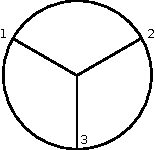
\includegraphics{img/chap7f4.pdf}
      \end{center}

      \vspace{5pt}
      There are three rotations: $0^\circ$, $120^\circ$ and $240^\circ$.
      There are three flips about the axes that are tangent to the 
      internal line segments. The permutations are

      \begin{align*}
          \eps &= \begin{pmatrix}
	             1 & 2 & 3 \\
		     1 & 2 & 3
		  \end{pmatrix}
		  &
	  f    &= \begin{pmatrix}
	             1 & 2 & 3 \\
		     2 & 3 & 1
		  \end{pmatrix}
		  \\
	  g    &= \begin{pmatrix}
	             1 & 2 & 3 \\
		     3 & 1 & 2
		  \end{pmatrix}
		  &
          h    &= \begin{pmatrix}
	             1 & 2 & 3 \\
		     1 & 3 & 2
		  \end{pmatrix}
		  \\
	  k    &= \begin{pmatrix}
	             1 & 2 & 3 \\
		     3 & 2 & 1
		  \end{pmatrix}
		  &
	  l    &= \begin{pmatrix}
	             1 & 2 & 3 \\
		     2 & 1 & 3
		  \end{pmatrix}
      \end{align*}

      And the table is 
      
      \begin{center}
      \begin{tabular}{c|cccccc}
         $\circ$ & $\eps$ & $f$ & $g$ & $h$ & $k$ & $l$ \\ \hline
         $\eps$  & $\eps$ & $f$ & $g$ & $h$ & $k$ & $l$ \\
	 $f$     & $f$ & $g$ & $\eps$ & $l$ & $h$ & $k$ \\
	 $g$     & $g$ & $\eps$ & $f$ & $k$ & $l$ & $h$ \\
	 $h$     & $h$ & $l$ & $k$ & $\eps$ & $g$ & $f$ \\
	 $k$     & $k$ & $h$ & $l$ & $f$ & $\eps$ & $g$ \\
	 $l$     & $l$ & $k$ & $h$ & $g$ & $f$ & $\eps$
      \end{tabular}
      \end{center}

   \end{enumerate}

   \item \textsc{Symmetries of Polynomials}

   \noindent Consider the polynomial $p=(x_1 - x_2)^2 + (x_3 - x_4)^2$.
   It is unaltered when the subscripts undergo any of the following
   permutations:

   \vspace{5pt}
   \begin{tabular}{cccc}
      \(\begin{pmatrix}
          1 & 2 & 3 & 4\\
	  2 & 1 & 3 & 4
        \end{pmatrix} \)
      &
      \(\begin{pmatrix}
          1 & 2 & 3 & 4\\
	  1 & 2 & 4 & 3
        \end{pmatrix} \)
      &
      \(\begin{pmatrix}
          1 & 2 & 3 & 4\\
	  2 & 1 & 4 & 3
        \end{pmatrix} \)
      &
      \(\begin{pmatrix}
          1 & 2 & 3 & 4\\
	  3 & 4 & 1 & 2
        \end{pmatrix} \)
   \end{tabular}

   \vspace{2pt}
   \begin{tabular}{cccc}
      \(\begin{pmatrix}
          1 & 2 & 3 & 4\\
	  4 & 3 & 1 & 2
        \end{pmatrix} \)
      &
      \(\begin{pmatrix}
          1 & 2 & 3 & 4\\
	  3 & 4 & 2 & 1
        \end{pmatrix} \)
      &
      \(\begin{pmatrix}
          1 & 2 & 3 & 4\\
	  4 & 3 & 2 & 1
        \end{pmatrix} \)
      &
      \(\begin{pmatrix}
          1 & 2 & 3 & 4\\
	  1 & 2 & 3 & 4
        \end{pmatrix} \)
   \end{tabular}

   \vspace{5pt}
   For example, the first of these permutations replaces $p$ by
   \[
      (x_2 - x_1)^2 + (x_3 - x_4)^2
   \]

   \noindent the second permutation replaces $p$ by 
   $(x_1 - x_2)^2 + (x_4 - x_3)^2$; and so on. The \emph{symmetries of
   a polynomial} $p$ are all the permutations of the subscripts which
   leave $p$ unchanged. They form a group of permutations.

   List the symmetries of each of the following polynomials, and write 
   their group table.

   \begin{enumerate}[1]
      \item $p=x_1x_2 + x_2x_3$

      \noindent \solution The symmetries are 

      \begin{align*}
         \eps &= \begin{pmatrix}
	            1 & 2 & 3 \\
		    1 & 2 & 3
		 \end{pmatrix}
		 &
	 f    &= \begin{pmatrix}
	            1 & 2 & 3 \\
		    3 & 2 & 1
		 \end{pmatrix}
      \end{align*}

      And the table is 
      \begin{tabular}{c|cc}
         $\circ$ & $\eps$ & $f$ \\ \hline
	 $\eps$  & $\eps$ & $f$ \\
	 $f$     & $f$ & $\eps$
      \end{tabular}

      \vspace{5pt}
      \item $p = (x_1 - x_2)(x_2 - x_3)(x_1 - x_3)$
      
      \noindent \solution It appears the subscripts 2 and 3 are 
      interchangeable. So the permutations are

      \begin{align*}
         \eps &= \begin{pmatrix}
	            1 & 2 & 3 \\
		    1 & 2 & 3
		 \end{pmatrix}
		 &
	 f    &= \begin{pmatrix}
	            1 & 2 & 3 \\
		    1 & 3 & 2
		 \end{pmatrix}
      \end{align*}

      And the table is 
      \begin{tabular}{c|cc}
         $\circ$ & $\eps$ & $f$ \\ \hline
	 $\eps$  & $\eps$ & $f$ \\
	 $f$     & $f$ & $\eps$
      \end{tabular}


      \vspace{5pt}
      \item $p=x_1x_2 + x_2x_3 + x_1x_3$

      \noindent \solution All subscripts are interchangeable. The
      permutations are

      \begin{align*}
         \eps &= \begin{pmatrix}
	            1 & 2 & 3 \\
		    1 & 2 & 3
		 \end{pmatrix}
		 &
	 f    &= \begin{pmatrix}
	            1 & 2 & 3 \\
		    1 & 3 & 2
		 \end{pmatrix}
	         \\
         g    &= \begin{pmatrix}
	            1 & 2 & 3 \\
		    2 & 1 & 3 
		 \end{pmatrix}
		 &
	 h    &= \begin{pmatrix}
	            1 & 2 & 3 \\
		    2 & 3 & 1
		 \end{pmatrix}
		 \\
	 k    &= \begin{pmatrix}
	            1 & 2 & 3 \\
		    3 & 1 & 2 
		 \end{pmatrix}
		 &
	 l    &= \begin{pmatrix}
	            1 & 2 & 3 \\
		    3 & 2 & 1
		 \end{pmatrix}
      \end{align*}

      And the table is

      \vspace{5pt}
      \begin{center}
      \begin{tabular}{c|cccccc}
        $\circ$ & $\eps$ & $f$ & $g$ & $h$ & $k$ & $l$ \\ \hline
	$\eps$  & $\eps$ & $f$ & $g$ & $h$ & $k$ & $l$ \\ 
	$f$     & $f$ & $\eps$ & $h$ & $g$ & $l$ & $k$ \\
	$g$     & $g$ & $k$ & $\eps$ & $l$ & $f$ & $h$ \\
	$h$     & $h$ & $l$ & $f$ & $k$ & $\eps$ & $g$ \\
	$k$     & $k$ & $g$ & $l$ & $\eps$ & $h$ & $f$ \\
	$l$     & $l$ & $h$ & $k$ & $f$ & $g$ & $\eps$
      \end{tabular}
      \end{center}

      \item $p=(x_1-x_2)(x_3-x_4)$
     
      \noindent \solution We can interchange subscripts 1 with 3 and 2 with 4.
      The permutations are

      \begin{align*}
         \eps &= \begin{pmatrix}
	            1 & 2 & 3 & 4 \\
	            1 & 2 & 3 & 4 
		 \end{pmatrix}
		 &
	 f    &= \begin{pmatrix}
	            1 & 2 & 3 & 4 \\
		    3 & 2 & 1 & 4 
		 \end{pmatrix}
		 \\
	 g    &= \begin{pmatrix}
	            1 & 2 & 3 & 4 \\
		    1 & 4 & 3 & 2
		 \end{pmatrix}
		 &
	 h    &= \begin{pmatrix}
	            1 & 2 & 3 & 4 \\
		    3 & 4 & 1 & 2
		 \end{pmatrix}
      \end{align*}

      And the table is

      \vspace{5pt}
      \begin{center}
      \begin{tabular}{c|cccc}
         $\circ$ & $\eps$ & $f$ & $g$ & $h$ \\ \hline
	 $\eps$  & $\eps$ & $f$ & $g$ & $h$ \\
	 $f$     & $f$ & $\eps$ & $h$ & $g$ \\
	 $g$     & $g$ & $h$ & $\eps$ & $f$ \\
	 $h$     & $h$ & $g$ & $f$ & $\eps$
      \end{tabular}
      \end{center}

   \end{enumerate}

   \item \textsc{Properties of Permutations of a Set} $A$

      \begin{enumerate}[1]
         \item Let $A$ be a set and $a \in A$. Let $G$ be the subset of
	 $S_A$ consisting of all the permutations $f$ of $A$ such that
	 $f(a)=a$. Prove that $G$ is a subgroup of $S_A$.

	 \noindent \solution Again we must show that $G$ is closed
	 with respect to $\circ$ and with respect to function 
	 inverses.

	 \hspace{.15in}Let $f$ and $g$ both be permutations that are in $G$.
	 Then $[f \circ g](a) = f(g(a)) = f(a) = a$. Therefore $f\circ g$ is in
	 $G$ and therefore $G$ is closed with respect to $\circ$.

	 \hspace{.15in}Again lets choose $f$ such that $f \in G$. We know that
	 $f(a)=a$.  We also know that there exists a function $g \in S_A$ that
	 is the inverse of $f$. We know this because $S_A$ is a group.  By the
	 definition of inverse we know that $y = f(x)$ iff $x = g(y)$. We know
	 that $f(a)=a$, therefore, $g(a)=a$. So $g$ is an inverse of $f$ and
	 $g \in G$, therefore $G$ is closed with respect
	 to inverses.

	 \hspace{.15in}Therefore, $G$ is a subgroup of $S_A$.

	 \item If $f$ is a permutation of $A$ and $a \in A$, we say that $f$
	 \emph{moves} $a$ if $f(a) \ne a$. Let $A$ be an infinite set, and
	 let $G$ be the subset of $S_A$ which consists of all the permutations
	 $f$ of $A$ which move \emph{only a finite number of elements} of $A$.
	 Prove that $G$ is a subgroup of $S_A$.

	 \solution Let $f,g \in G$. Then $f$ and $g$ move only a finite 
	 number of elements. Assume $f$ moves the elements $a_1, a_2, \dots,
	 a_n$ and $g$ moves the elements $b_1, b_2, \dots, b_m$. Then for
	 any element $x \in A$ which is not in $\{a_1, a_2, \dots, a_n, b_1,
	 b_2, \dots, b_m\}$ we have
	 
	 \begin{align*}
	    [f \circ g](x) &= f(g(x)) \\
	                   &= f(x)    \\
			   &= x
	 \end{align*}

	 Hence, at most $[f \circ g]$ moves the finite set of elements
	 $\{a_1, a_2, \dots, a_n, b_1, b_2, \dots b_m\}$. Therefore,
	 $[f\circ g] \in G$ and $G$ is closed with respect to $\circ$.

	 Next, assume $f \in G$. Then $f$ moves a finites number of elements.
	 Assume it contains the following moves:
	 \begin{align*}
	    f & = \begin{pmatrix}
		      a_1 & a_2 & \cdots & a_n  \\
		      b_1 & b_2 & \cdots & b_n 
		  \end{pmatrix} \\
	 \end{align*}

	 Then $f^{-1}$ is the function
	 \begin{align*}
	    f & = \begin{pmatrix}
		      b_1 & b_2 & \cdots & b_n \\
		      a_1 & a_2 & \cdots & a_n  
		  \end{pmatrix} \\
	 \end{align*}

	 and $f^{-1}$ only moves a finite number of elements. Therefore
	 $G$ is closed with respect to inverses.

	 \hspace{.15in}Therefore $G$ is a subgroup of $S_A$.

	 \item Let $A$ be a \emph{finite} set, and $B$ a subset of $A$.
	 Let $G$ be the subset of $S_A$ consisting of all the permutations 
	 $f$ of $A$ such that $f(x) \in B$ for every $x \in B$. Prove that
	 $G$ is a subgroup of $S_A$.

	 \solution Assume $f,g \in G$. Then for every $x \in B$ we have
	 $f(x) \in B$ and $g(x) \in B$. So now take any $x \in B$.
	 Then $g(x) \in B$ and $f(g(x)) \in B$. Therefore $[f \circ g] \in G$.
	 Therefore $G$ is closed with respect to $\circ$.
	 
	 Again assume that $f \in G$. Then $f(x) \in B$ if $x \in B$.
	 Since $A$ is finite we know that $B$ is finite. And we know that
	 $f$ is bijective and has an inverse $f^{-1}$. Since it is bijective
	 (like all permutations) we know that
	 if $x \in B$ then $f^{-1}(x) \in B$.
	 Therefore $f^{-1}$ is in $G$
	 and $G$ is closed with respect to inverses. Therefore $G$ is
	 a subgroup of $S_A$.
         

	 \item Given an example to show that the conclusion of part 3
	 is not necessarily true if $A$ is an infinite set.

	 \solution Let $A$ be \Integers. Let $B$ be $\Integers^+$. So
	 we have $B \subset A$. Let $f$ be the function $f(x) = x + 1$
	 For any value $x \in B$ we know $f(x) \in B$ (adding 1 to any
	 positive integer results in a positive integer). However, the inverse
	 of $f$ is $f^{-1}(x) = x - 1$. Now look at $f^{-1}(1) = 0$ and
	 we have a case where $x \in B$ but $f^{-1}(x) \notin B$.
	 Therefore $f^{-1} \notin G$ and therefore $G$ is not closed
	 with respect to inverses and is not a subgroup of $S_A$.


	 The key difference is that the function $f$ is bijective in $A$
	 but not in $B$.

	    

      \end{enumerate}
 
\end{enumerate}

\end{document}
